\chapter{Control of a Mobile Manipulator }
\label{c5_Control}
In this chapter, the control architecture of the tele-operated  mobile manipulator or platform  is presented. The user interface for teleoperation is discussed. The control algorithm  running on the mobile manipulator and the hardware used for the control of traction and steering is discussed. The protocol used  for communication between the robot and the user interface is also described in detail.
\section{Control Architecture and Hardware}


\begin{figure}
	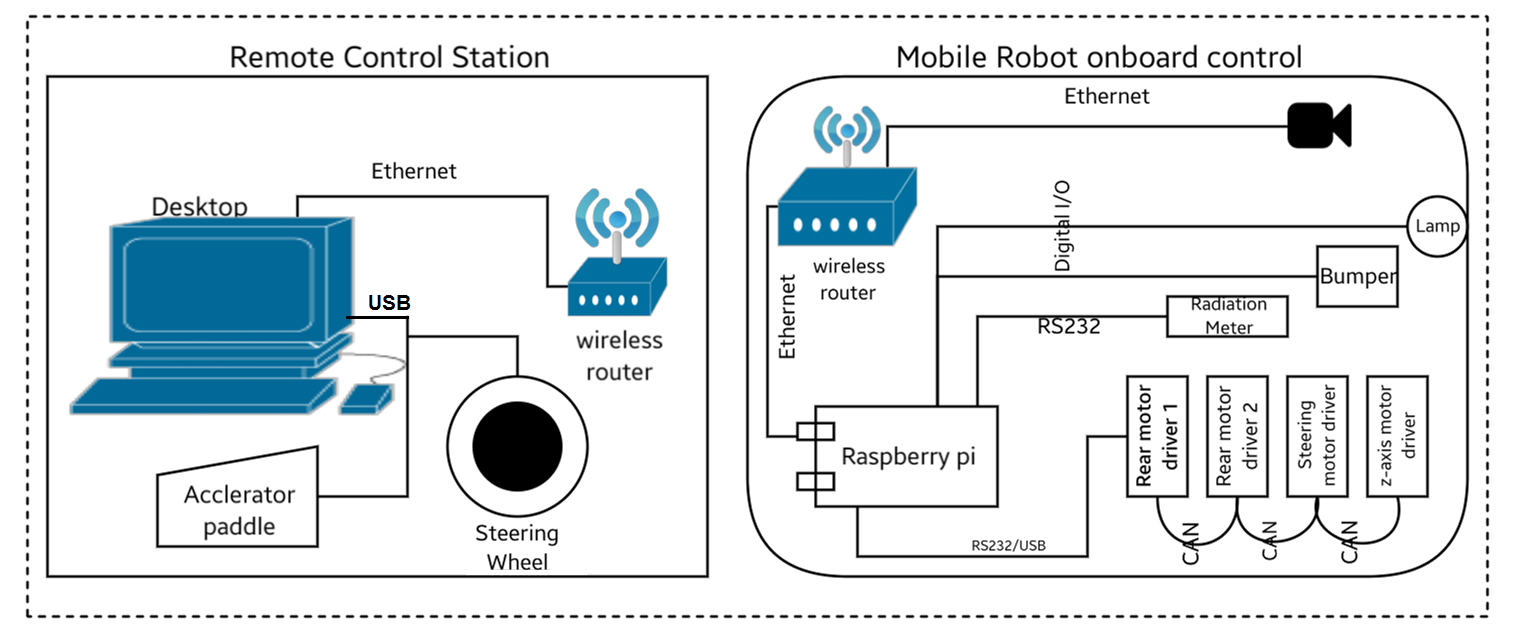
\includegraphics[width=\linewidth,keepaspectratio]{Chapter3/fig/controlblock}
	\captionof{figure}{Control architecture }
	\label{fig:ControlBlockDiag} 
\end{figure} 
The mobile manipulator explained in chapter \ref{ch_3:Design} was planned to be teleoperated over a wireless network. The control block diagram and architecture are shown in Figure \ref{fig:ControlBlockDiag}. It has a remote control station which is the interface for the operator and a local onboard controller of the mobile robot. They  communicate over a dedicated wireless network. The remote station sends data packet in every  50 milliseconds (20Hz) to the mobile robot. The commanded velocity, steer angle,  z position of the platform, and  state of the detector and headlamps constitute the data packet sent by the remote station, as shown in Figure \ref{fig:sentBytes}. The onboard controller of the mobile robot replies with a data packet consisting of the $X$, $Y$ position and orientation $\theta$ of the robot, the current steer angle, angular velocities of each wheel, the z position of the top platform,  battery voltage  and current of each motor. They are indicated in Figure \ref{fig:recvBytes}.
\begin{figure}
	
	\begin{minipage}[t]{0.5\textwidth}
		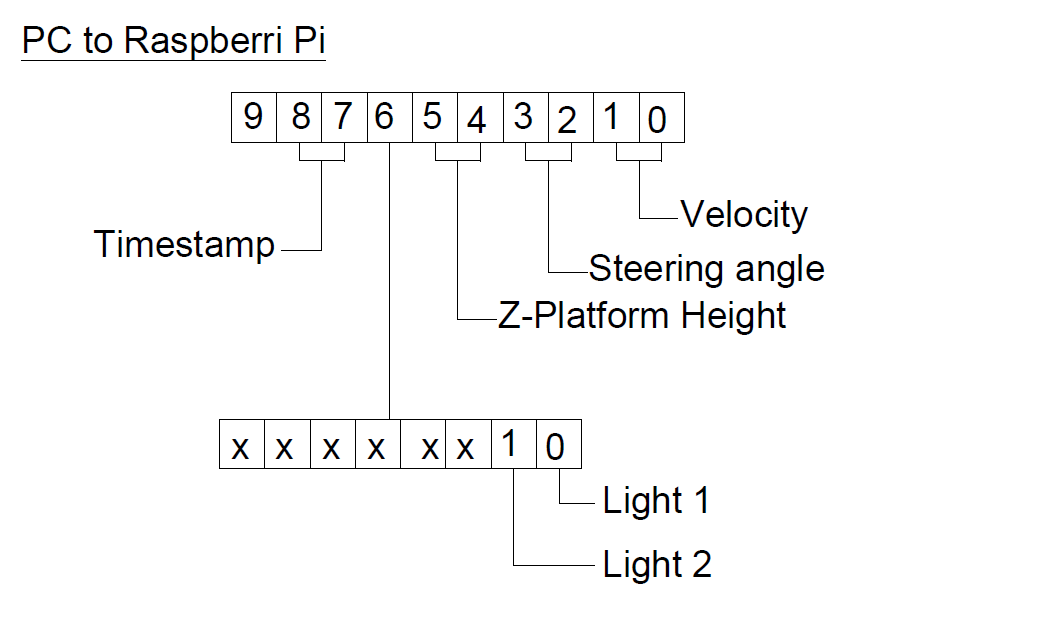
\includegraphics[width=\linewidth,keepaspectratio]{Chapter5/fig/bitconfig}
		\captionof{figure}{Data from PC to the robot }
		\label{fig:sentBytes} 
	\end{minipage}
\hfill
   \begin{minipage}[t]{0.5\textwidth}
   		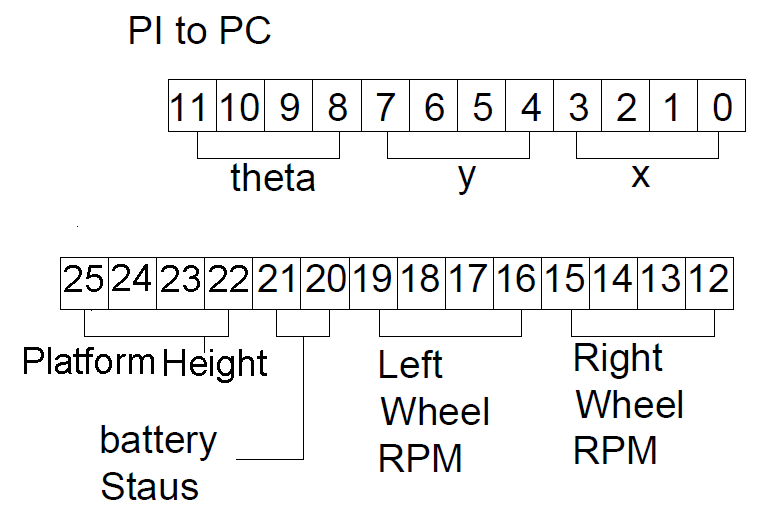
\includegraphics[width=\linewidth,keepaspectratio]{Chapter5/fig/bitconfig2}
   		\captionof{figure}{Data from the robot to PC}
   		\label{fig:recvBytes} 
   \end{minipage}
	
\end{figure}

\subsection{Local onboard controller}
The  onboard computer which is Raspberry Pi running Raspian (linux) OS receives  command from the remote station and controls the robot hardware through customized C++ application.
The Raspberry Pi  is daisy chained to the four Maxon make, EPOS2 motor controllers/drivers. The communication between the onboard computer and the first Maxon controller is over usb/RS232 interface using Maxon's proprietorial protocol~\cite{maxonrs232}. The first controller serves as CAN master for the rest of the controllers. The rear wheel motor drivers were configured in velocity servo loop. The drivers for steering and the z-axis motors were configured in position control loop.  The camera mounted on the mobile robot  and Raspberry Pi  were connected over Ethernet via a wireless hub. The wiring diagram of the robot is given in Figure \ref {fig:wiring}. Since the onboard camera is connected to the wireless network directly, it does not interfere with the command loop between the Raspberri Pi and the PC. 
\begin{figure}
	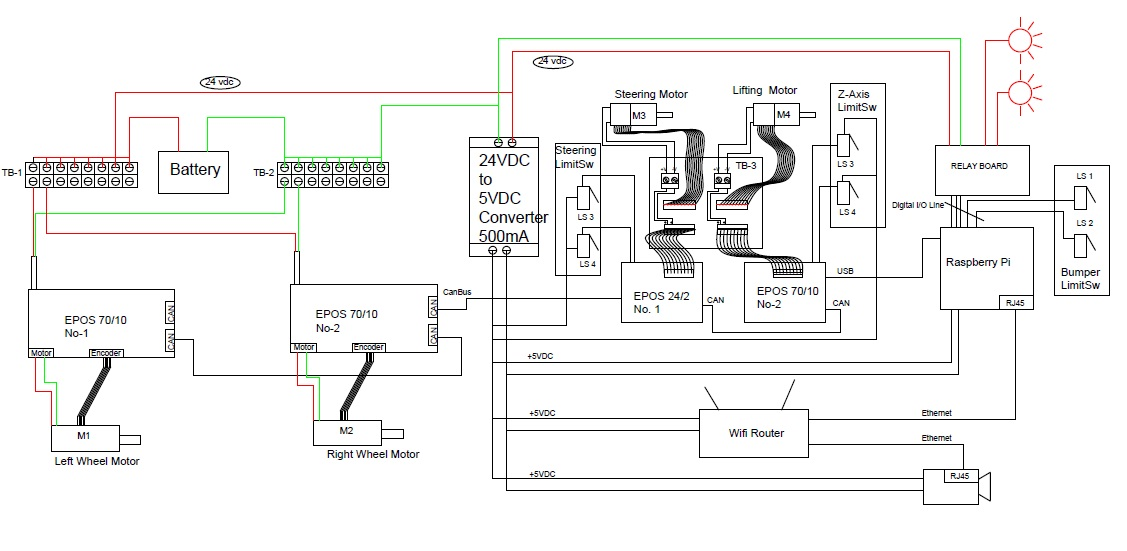
\includegraphics[width=\linewidth,keepaspectratio]{Chapter5/fig/RobotSideWiring}
	\captionof{figure}{Wiring  diagram of the WMR }
	\label{fig:wiring} 
\end{figure} 

The mobile robot is teleoperated using position-speed command as in \cite{farkhatdinov2007hybrid}.  The workspace for the mobile robot was assumed  infinite compared to the input device. In case of manipulators position-position, control approach is generally used with scaling. In this case,  the mixed approach was used. The steering angle was controlled in position-position mode whereas the mobile robot's speed was controlled by foot pedal's position, i.e. in  position-velocity mode. This can be given by the following equation: 
\begin{equation}
	\begin{pmatrix}
	V\\\theta_S
	\end{pmatrix}=
	\begin{pmatrix}
	K_v & 0\\0 & K_s
	\end{pmatrix}
	\begin{pmatrix}
	\tilde{X_p}\\
	\tilde{\Theta_s}
	\end{pmatrix}
\end{equation}
where $\tilde{X_p}$ is the displacement of pedal, $\tilde{\theta_s}$ is the twist of steering wheel, $K_v$ and $K_s$ are the proportionality constants, $V$ is the velocity of point $O_3$   and $\theta_s$ is the displacement of the steer motor. These proportionality constants are derived  based on extreme limits. They are  listed in Table \ref{tbl:propCnst}. 

\begin{table}[!htbp]
	\caption{Proportionality constant table} 
	\label{tbl:propCnst}
	\centering
	\begin{tabular}{l l l l l}
		\hline
		Robot  & range & Joy-Stick& range & parameter \\
		parameters& & Parameter & & Value\\
		\hline
		$\theta_s$ & -60 to +60 & $\tilde{\Theta_s}$ & $-90^o$ to $90^o$ & $K_s=2/3$\\
		$V$ & 0 to +60 mm/sec & $\tilde{X_p}$ & 0 to 30mm & $K_v=2$\\
		\hline
	\end{tabular}	
\end{table}


\subsection{Details of the motor controller}
Three EPOS2 controllers from Maxon Motors were used to control the mobile robot's rear wheel velocity and the steering gears position. Each controller can control one motor. The overall architecture of the controller  as given in \cite{maxonAutoTune}, \cite{maxonAppNotesPosition}  is shown  in  Figure \ref{fig:EPOS4}.
  \begin{figure}
	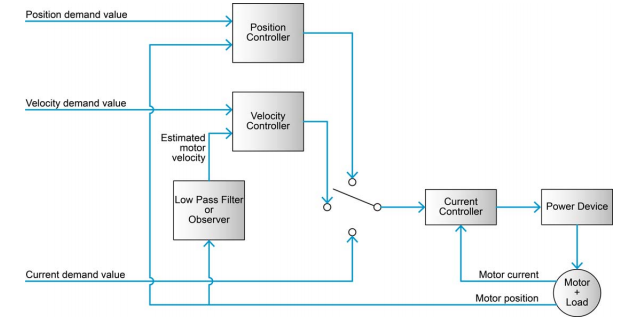
\includegraphics[width=\linewidth,keepaspectratio]{Chapter5/fig/overallcontorl}
	\captionof{figure}{Block diagram of EPOS4 controller  }
	\label{fig:EPOS4} 
\end{figure}
 The controller can be configured in either current, position or velocity control mode. The inner most current loop controls the torque of the motor.
 The current feedback loop shown in Figure \ref{fig:curloop} is a Proportional Integrator (PI) controller, running at 25KHz and the transfer function of the PI block is given as \ref{eqn:curLoop}. 
 \begin{equation}
 	C(s)=K_p + \frac{K_I}{s}
 	\label{eqn:curLoop}
 \end{equation}
 where $K_p$ and $ K_I$ are the proportional and integral gains.
 
 
 \begin{figure}
 	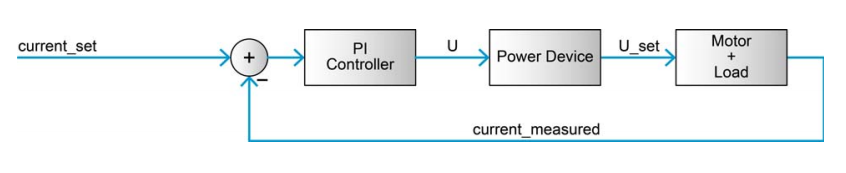
\includegraphics[width=\linewidth,keepaspectratio]{Chapter5/fig/currentLoop}
 	\captionof{figure}{Current control block }
 	\label{fig:curloop} 
 \end{figure}
 
 
  The rear motor controllers are configured in the velocity control mode.  The block digram  of the velocity loop is given in Figure \ref{fig:velloop}. The velocity controller is a PI controller with  velocity and acceleration feed-forward. 
  \begin{figure}
  	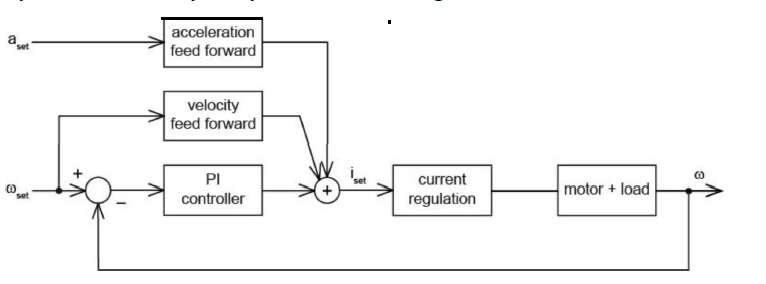
\includegraphics[width=\linewidth,keepaspectratio]{Chapter5/fig/velLoop}
  	\captionof{figure}{Velocity control bolck  }
  	\label{fig:velloop} 
  \end{figure}
  The transfer function $V(s)$ of the velocity loop PI block is given by
  \begin{eqnarray}
  V(s)=K_{p\omega}+\frac{K_{I\omega}}{s}
  \end{eqnarray}  where $K_{p\omega}$ and  $K_{I\omega}$ are  proportional and integral gains for velocity, respectively.   The sampling rate of the  velocity loop is 2.5 KHz. The feedforward acceleration and  velocity was used to compensate for the known inertial load and  viscous frictional load  \cite{maxonAppNotesPosition} respectively.   Velocity is estimated from differentiation of  the position data, the low-pass filter  in Figure \ref{fig:EPOS4}  eliminates noise due to differentiation. The transfer function $H(s)$ for the  low-pass filter is given by
  \begin{equation}
  H(s)=\frac{1}{1+\frac{K_{p\omega}}{48K_{I\omega}}}
  \end{equation} 
  
  The gain values used for each rear motor in  the velocity control mode is listed in Table \ref{tb:motorPara}. No acceleration or velocity feedforward  was used. The gain parameters were determined by auto tuning software provided by Maxon Motors.  
  

  	  \begin{table}[!htbp]
  		\caption{Parameters for left and right rear wheel motor controllers  }
  		\label{tb:motorPara}
  		\centering
  		\begin{tabular}{c c c c}
  			\hline
  			\emph{Gain}  & \emph{ Right motor}  & \emph{ Left motor}& \emph{Unit} \\
  			\emph{ Parameter}  & \emph{ Value} & \emph{ Value} & \emph{\space} \\
  			\hline
  			$K_p$  & 300 & 230 &  $\frac{mV}{A}$ \\ 
  			$K_I $ & 100 & 53 & $\frac{mV}{A.mS}$ \\
  			$K_{P\omega}$& 1000 & 5182 & $ \frac{mA.sec}{rad}$\\
  			$K_{I\omega}$&100 & 425& $\frac{mA}{rad}$\\
  			\hline
  		\end{tabular}
  	\end{table}






The steering motor is in position control mode. The block digram is shown in Figure \ref{fig:posloop}. It is a PID controller with transfer function given as 
\begin{equation}
P(s)=K_{PP}+K_{IP}s+\frac{K_{DP}s}{1+\frac{K_{DP}}{10 K_{PP}}s}
\end{equation}
where $K_{PP}$, $K_{IP}$ and $K_{DP}$ are position proportional, integral and derivative gains respectively. The velocity feed-forward $F_{\omega P}$ and acceleration feed-forward $F_{\alpha P}$ were used in position control loop to take care of viscous friction and known inertial load. The gains for controller were decided using auto tuning software provided by Maxon Motors. The values are reported in Table \ref{tb:steer}.

 It may be noted that the controller parameters listed in Table \ref{tb:steer} are very different from those used in simulation. This difference is due to the fact that the control structures are different. In the actual system motor dynamics influences, which was not considered during the simulation. In simulation,  position error directly affects the torque of the motor through the control parameters $K_p$, $K_d$ and $K_I$, whereas the position error in actual system sets  the motor current. Hence their units too are different. Direct comparison between simulation PID parameters and actual controllers PID values cannot be done. However, the PID parameters tuned during simulation provided a starting point for the PID tuning for the actual system.  
\begin{figure}
	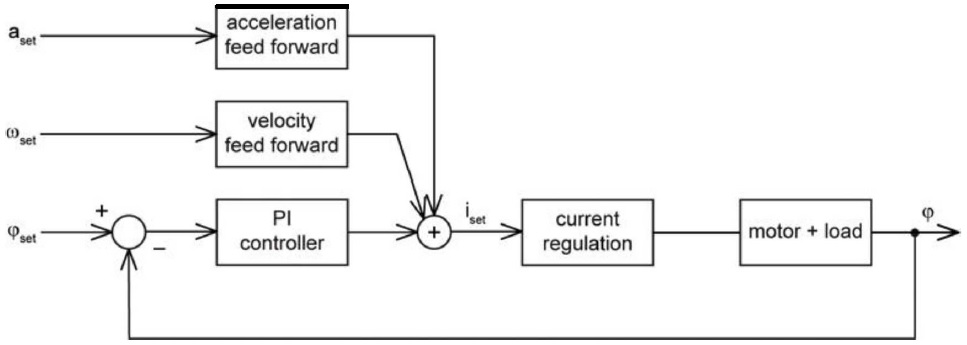
\includegraphics[width=\linewidth,keepaspectratio]{Chapter5/fig/posLoop}
	\captionof{figure}{Position control bolck  }
	\label{fig:posloop} 
\end{figure}
\begin{table}[!htbp]
	\caption{ Parameters of steering motor controller }
	\label{tb:steer}
	\centering
	\begin{tabular}{l l l}
		\hline
		\emph{Gain Parameter}  & \emph{ Value} & \emph{Unit} \\
		\hline
		$K_p$  & 537 &  $\frac{mV}{A}$ \\ 
		$K_I $ & 307 & $\frac{mV}{A.mS}$ \\
		$K_{PP}$& 128 & $ \frac{mA.sec}{rad}$\\
		$K_{IP}$&663&$\frac{mA}{rad}$\\
		$K_{ID}$&200&$\frac{mA}{rad}$\\
		$F_{\omega P}$& 0& $ \frac{mA.sec}{rad}$\\
		$F_{\alpha P}$& 54& $ \frac{mA.sec^2}{rad}$\\
		\hline
	\end{tabular}
\end{table}
\section{Control Algorithm }
This section discusses in detail the algorithm running on the onboard controller.  Command received by the controller was parsed to extract the velocity  and the steer angle  information. They were suitably scaled to get command velocity  $V$ in mm/sec, and steering  angle $\theta_s$ in radians.  It may be noted that the velocity $V$ corresponds to the velocity of point $O_r$ the reference point of the mobile robot.  Next the set point for each motor was calculated  and sent to individual drive. The algorithm is listed below and the block digram for the same in Figure \ref{fig:ControlBlock}
\begin{figure}[h]
	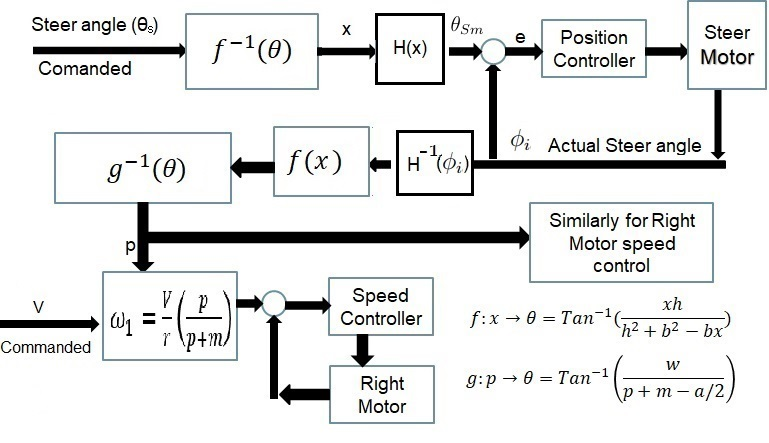
\includegraphics[width=\linewidth,keepaspectratio]{Chapter5/fig/BlkDigLocal2}
	\captionof{figure}{Block diagram of WMR controler}
	\label{fig:ControlBlock} 
\end{figure}

\begin{enumerate}
	\item Calculate the setpoint for steering motor $\theta_{SM} $ based on $\theta_s$.
	\item Read the current steering  angle $\phi_{ic}$.
	\item Calculate the velocity setpoints $\omega_{i}$ and $\omega_{o}$ of  rear wheels based on the $V$ and $\phi_{ic}$.

	
	\item Command  setpoints $\omega_{i}$, $\omega_{o}$ and $\theta_{SM} $ to each motor. 
\end{enumerate}
The above loop is repeated every 50 mSec.

It may be noted that the steer angle command received from the control station is not directly sent to the steer motor as set point after suitable scaling. The steer set point is based on the current rear wheel velocities. This is important as the response time of the  motors are different. The above methodology helps  minimize the deviation  from the Ackerman  steering condition even during transit condition, particularly, in case of large change in commanded $v$ and $\theta_s$. 
Each block in Figure \ref{fig:ControlBlock} is discussed next. 

 It may be noted that the $\theta_s$ always refers to the steer angle of the inner front wheel $\phi_i$  and $V$ refers to $O_r$ as shown in Figure \ref{fig:KenVec}, i.e.
 \begin{equation}
	 \theta_s =\phi_i
 \end{equation}
 The set point of the steering motor at the output of  gear box $\theta_{SM}$ is given by equations \ref{eqn:sterineq1} and \ref{eqn:sterineq2}  based on the geometry of Davis steering gear \cite{TOMBook}.
\begin{equation*}
 \tan\phi_i=\frac{xh}{h^2+b^2-bx}
\end{equation*}
or
\begin{eqnarray}
f(\phi_i): x=\frac{\tan\phi_i (h^2+b^2)}{h+b \tan\phi_i }
\label{eqn:sterineq1}
\end{eqnarray}
\begin{figure}
	\begin{minipage}[t]{0.6\textwidth}
		\centering
		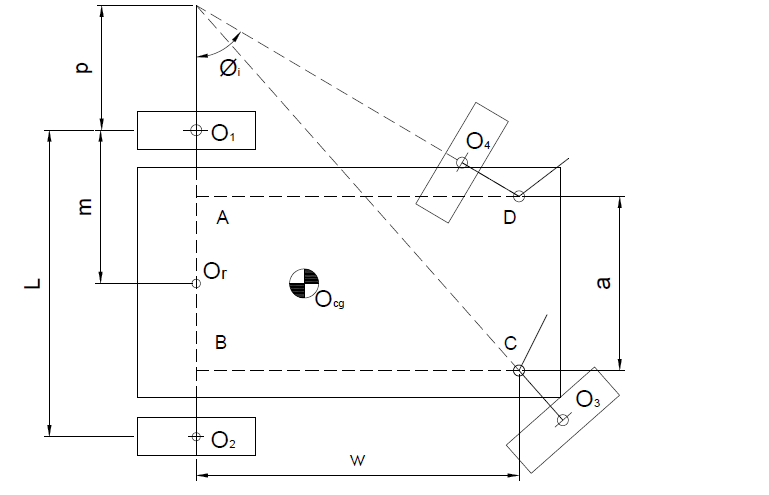
\includegraphics[width=5in]{Chapter5/fig/kinvec} 
		\caption{Ackerman steering condition}\label{fig:KenVec}
	\end{minipage}
	%\hfill
	\begin{minipage}[t]{0.7\textwidth}
		\centering
		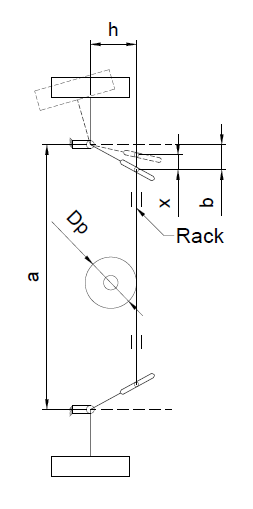
\includegraphics[height=3.5in]{Chapter5/fig/davisgear} 
		\caption{Davis steering gear}\label{fig:steering_gear_train}
	\end{minipage}
\end{figure}
where $x$ is the displacement of the rack and $h$ and $b$ are link lengths. The rack is connected to the steering motor by pinion of PCD $D_p$ (30mm) as shown in  Figure \ref{fig:steering_gear_train}. Therefore, the steering motor angle,  $ \theta_{Sm}$, is given below as
\begin{eqnarray}
H(x): \theta_{Sm}= x \frac{360}{\pi D_p}
\label{eqn:sterineq2}
\end{eqnarray}
 
Next,  the equation relating current steer angle $\phi_{i}$   and rear wheel  set point velocities $\omega_{RS}$ and $\omega_{LS}$ is presented. From the geometry of Figure \ref{fig:KenVec}, one gets
\begin{align}
\nonumber \tan\phi_{i} &=\frac{\bar{BD}}{\bar{OB}}=\frac{w}{p+m-a/2}\\ 
g:\phi_{i} \rightarrow p,\quad \quad p &= \frac{w}{\tan\phi_{i}}-m + \frac{a}{2}
\label{eqn:pFromTheta}
\end{align}
%similarly for the inner wheel we get  
%\begin{equation}
%p = \frac{w}{\tan\theta_i}-m - \frac{a}{2}
%\end{equation}
Now using Equations \ref{velO1} and \ref{omegaPlat}  in equations relating the right and left wheel velocities to the WMR platform angular velocity $\omega_3$ and velocity, $V$, of the reference point $O_r$, presented below
\begin{align*}
\dot{O_r}&=\dot{O_i}+\omega_3 \times (O_r-O_i)\\
\dot{O_r}&=\dot{O_o}+\omega_3 \times (O_r-O_o)
\end{align*}
 We get the  velocity of each rear wheel as  
\begin{align}
\nonumber \omega_i&=\frac{Vp}{r(p+m)}\\
\nonumber \omega_o &=\frac{V(p+2m)}{r(p+m)}
\end{align}
Using the above equations and Equation \ref{eqn:pFromTheta},  the setpoints for the rear wheels are as follows 
\begin{equation}
\omega_i =\frac{V}{r}\frac{( \frac{w}{\tan\theta_o}-m + \frac{a}{2})}{ \frac{w}{\tan\theta_o}-m + \frac{a}{2}+m}
\end{equation}
\begin{equation}
\omega_o =\frac{V}{r}\frac{( \frac{w}{\tan\theta_o}-m + \frac{a}{2})+2m}{ \frac{w}{\tan\theta_o}-m + \frac{a}{2}+m}
\end{equation}
 

 
%\begin{itemize}
%\item calibration of steer data and wheel velocity
%\end{itemize}
\subsection{Safety interlocks}
The control algorithm has safety interlocks built into it. The vehicle speed has been limited to $0.5$ m/sec, this was done based on operator feedback for convenience in driving the vehicle remotely. The vehicle does not move if the manipulator is in the extended condition. This is to avoid overturning of the vehicle in case it has to climb a ramp. Acceleration of the vehicle is never exceeded beyond the limiting value of  $0.144g$ which was arrived at  based on dynamic stability of the mobile robot as calculated in Equation \ref{eqn:overturn}. To avoid overturning of vehicle while following a circular path, the linear velocity of the vehicle is limited by Equation \ref{eqn:Vel_limit} which is a function of the turning radius.
\subsection{Wheel odometery }
The dead reckoning odometery can be performed based on either the differential drive or Bicycle model. In the present case, we use the differential drive model. Where the rear wheel velocities were used to determine the position and orientation of the mobile robot. The position here means the position of the reference point $O_r$. The steps are followes.
\begin{enumerate}
	\item calculate $V$ and $\omega_3$ from current wheel velocities $\omega_1$  and  $\omega_2$  using equations \ref{omegaPlat} and \ref{velPlat} with $a=0$.
	\item integrate $V$ and $\omega_3$ over time step.
\end{enumerate}
If $x(t)$, $y(t)$ are the coordinate of $O_r$  and  $\beta(t)$ be the orientation of the robot with some global coordinate system, the kinematic model of the differential wheel robots is given by \cite{campion1996structural}  
\begin{equation}
\label{eqn:DiffKinModel}
\begin{pmatrix}
\dot{x}\\\dot{y}\\\dot{\beta}
\end{pmatrix}=
\begin{pmatrix}
\cos\beta & 0\\
\sin\beta & 0\\
0&1
\end{pmatrix}
\begin{pmatrix}
V\\\omega_3
\end{pmatrix}
\end{equation}
Equation \ref{eqn:DiffKinModel} is numerically integrated for time $\delta t$ using the following expressions:
\begin{align}
\label{eqn:odo1}
 x(i+1)&=x(i)+\delta t~ V(i)\cos\beta(i);\\
 \label{eqn:odo2}
y(i+1)&=y(i)+\delta t~V(i)\sin\beta(i);\\
\label{eqn:odo3}
\beta(i+1)&=\beta(i)+\delta t~\omega_3(i);
\end{align}
where $i$ is at time step $t_i$. Next,  the actual odometric results for the vehicle moving in a circle and a straight line are presented.
\begin{figure*}
	\begin{minipage}[t]{0.5\textwidth}
		\centering
		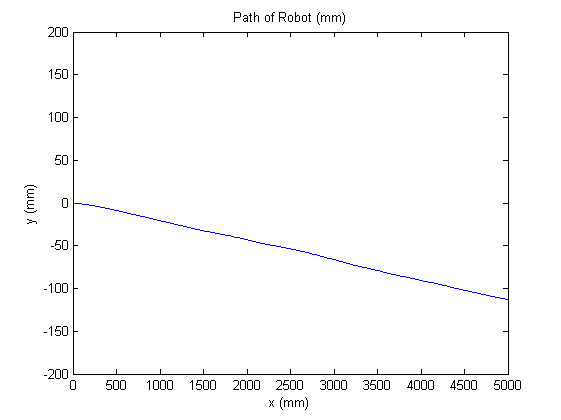
\includegraphics[width=3.0in]{Chapter5/fig/Line} 
		\caption{Tracing a line}\label{fig:line}
	\end{minipage}
	\hfill
	\begin{minipage}[t]{0.5\textwidth}
		\centering
		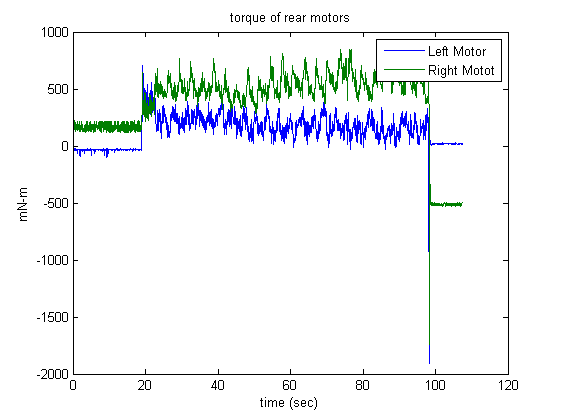
\includegraphics[width=3.2in]{Chapter5/fig/linTorq} 
		\caption{Motor torque}\label{fig:linTorq}
	\end{minipage}
	\begin{minipage}[t]{0.5\textwidth}
		\centering
		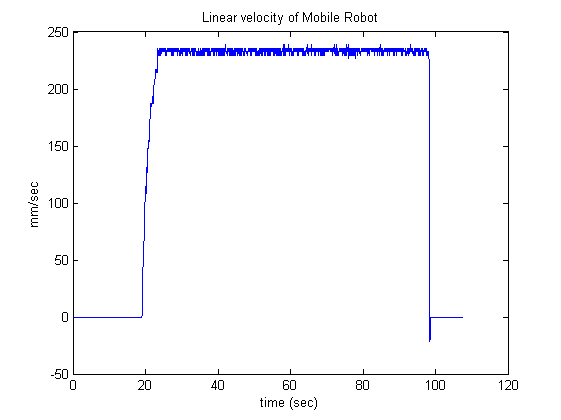
\includegraphics[width=3.1in]{Chapter5/fig/linVel} 
		\caption{Linear velocity}\label{fig:linVel}
	\end{minipage}
	\hfill
	\begin{minipage}[t]{0.5\textwidth}
		\centering
		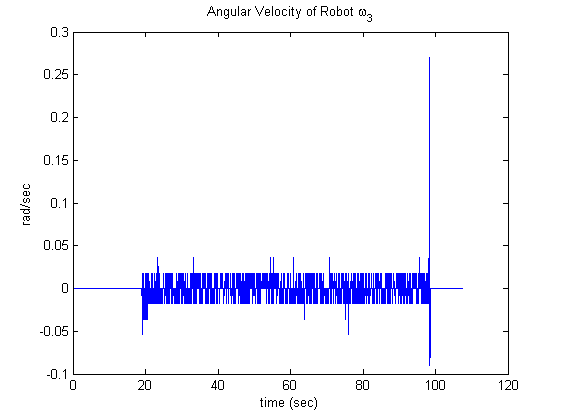
\includegraphics[width=3.1in]{Chapter5/fig/linOmega} 
		\caption{Angular velocity}\label{fig:linOmega}
	\end{minipage}
	%\caption{Linear motion of  WMR}
\end{figure*}

As seen in the graph of Figure \ref{fig:line} there is a lateral shift in the robots path calculated using odometry.  There is a linear shift too, which can observed due to longer path calculated by odometry. The lateral shift of 200 mm and a linear shift of 300 mm for 15000 mm long path was calculated. This clearly indicates slip in the wheels. The torque curves also shows that one wheel is more loaded that the other this is expected as the battery weight was on one side of the robot.

In Figure \ref{fig:cirVel} the robot traces circular path of two different radius. It can be seen that there is no lateral (side) slip during the motion. The step change in the angular velocity at time $ t\approx125~sec$, shown in Figure \ref{fig:cirOmega}, indicate transition to a larger radius path. The linear velocity of the robot is maintained constant at $ 300~mm/sec$.
\begin{figure}
	\begin{minipage}[t]{0.5\textwidth}
		\centering
		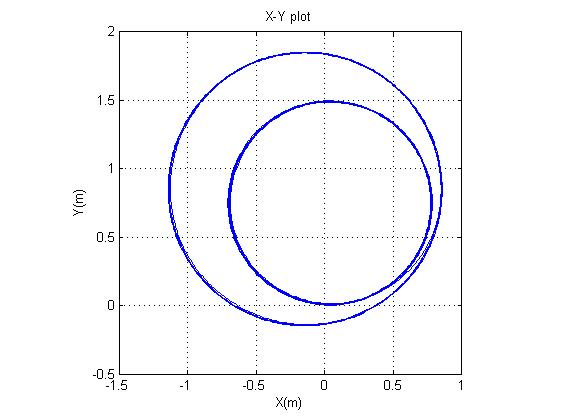
\includegraphics[width=3.5in]{Chapter5/fig/CircleOdo} 
		\caption{Tracing a circle}\label{fig:circle}
	\end{minipage}
	\hfill
	\begin{minipage}[t]{0.5\textwidth}
		\centering
		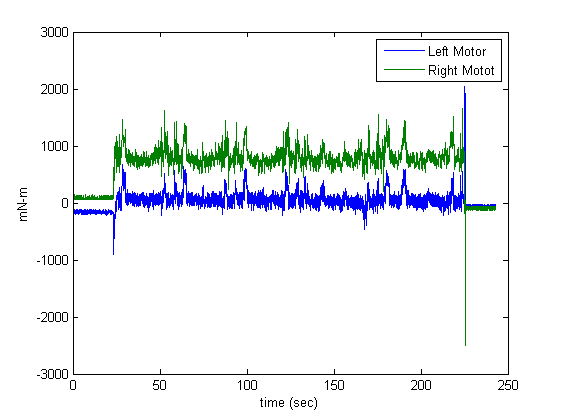
\includegraphics[width=3.2in]{Chapter5/fig/cirTorq} 
		\caption{Motor torque}\label{fig:cirTorq}
	\end{minipage}
\vfill 
\begin{minipage}[t]{0.5\textwidth}
	\centering
	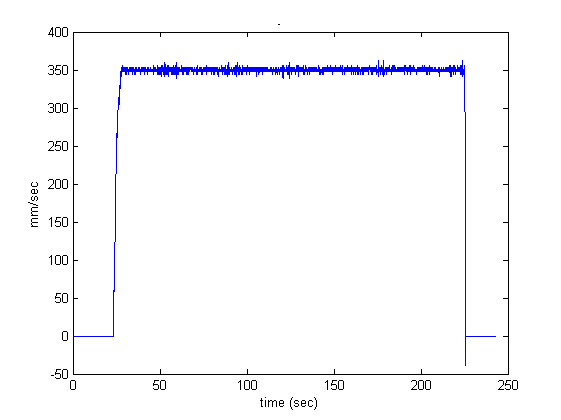
\includegraphics[width=3.1in]{Chapter5/fig/cirVel} 
	\caption{Linear velocity}\label{fig:cirVel}
\end{minipage}
\hfill
\begin{minipage}[t]{0.5\textwidth}
	\centering
	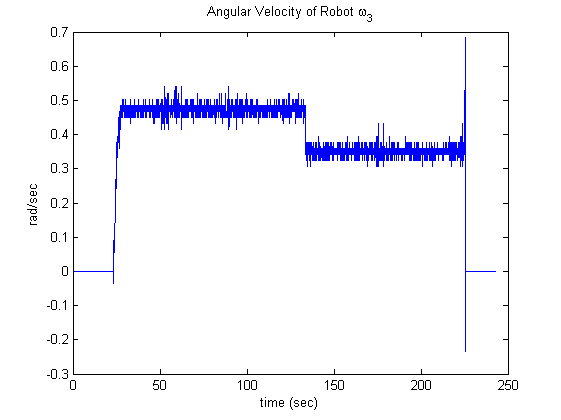
\includegraphics[width=3.1in]{Chapter5/fig/cirOmega} 
	\caption{Angular velocity}\label{fig:cirOmega}
\end{minipage}
	%\caption{Circular motion of  WMR}
\end{figure}

\section{ Remote control station}   
The operator controls the vehicle from a local station away from the robot over a wireless network. The control station consists of a desktop computer running Windows XP. A steering wheel and two foot switches are connected to the desktop. The steering wheel sets the steering of the remote mobile robot and the footpadel is used to set the velocity $V$ of the robot. A push button in the steering wheel is used to reverse the direction of motion of the robot.

The screen of the desktop displays  video streaming  from the mobile robot's on board camera. A graphical user  interface (GUI) shown in Figure \ref{fig:Gui} displays the robot's parameters such as current steer angle, velocity of each rear wheels and the position of the z-axis. Buttons on the GUI operates the z-axis, head lamps, etc.

\begin{figure}
	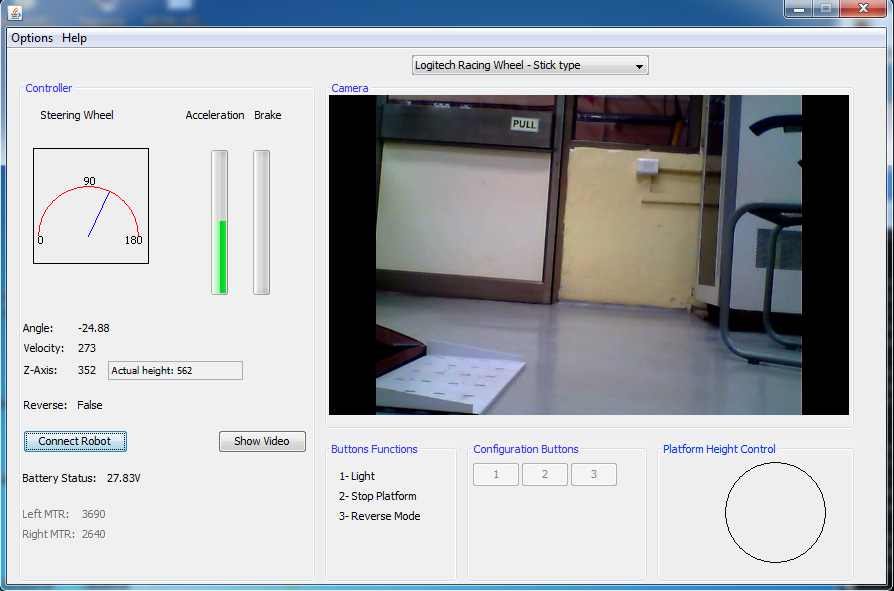
\includegraphics[width=\linewidth,keepaspectratio]{Chapter5/fig/gui}
	\captionof{figure}{User interface for teleoperation }
	\label{fig:Gui} 
\end{figure}


%\subsubsection{Control of Z platform}
%Decentralized control technique treats the manipulator and the platform as two different system. The inter-coupling forces are treated as external forces on the system. The dynamics equation of the mobile manipulator can thus be split as follows [3].
%\section{Admissible path}
%\section{Trajectory Tacking}


\section{Summary}
In this chapter, the control architecture of the mobile manipulator has been presented. The  algorithm used  to move the robot was discussed in detail. The odometry used for pose estimation of the robot was also presented with the experimental results. 

